Cells are the fundamental unit for all life on Earth. In order
for them to perform their biological tasks, the complex structures they contain
must be able to replicate and move within their aqueous environment. This
transport problem  poses a unique challenge as diffusion alone is far to slow,
and random, a process to be able to produce movement on cellular timescales[].
Nature's solution to this problem is twofold. Within each cell there is a vast network of interweaving filaments called the \textit{cytoskeleton} that spans the gaps between the substructures of the cell. This cytoskeleton serves as a highway to a class of proteins called \textit{molecular motors} which can be distinguished into three types: kinesin, myosin, and dynein. Molecular motors attach to cellular cargo and drag it along the cytoskeleton by hydrolyzing Adenosine triphosphate (ATP) in order to convert stored chemical energy into mechanical work\cite{alberts_molecular_2002}. Correct operation of these motors results in processes such as cell division, muscle contraction, and axonal transport; failure can lead to debilitating diseases such as ALS \cite{boillee_als:_2006}. 

\begin{figure}[!hbt]
	\centering 
	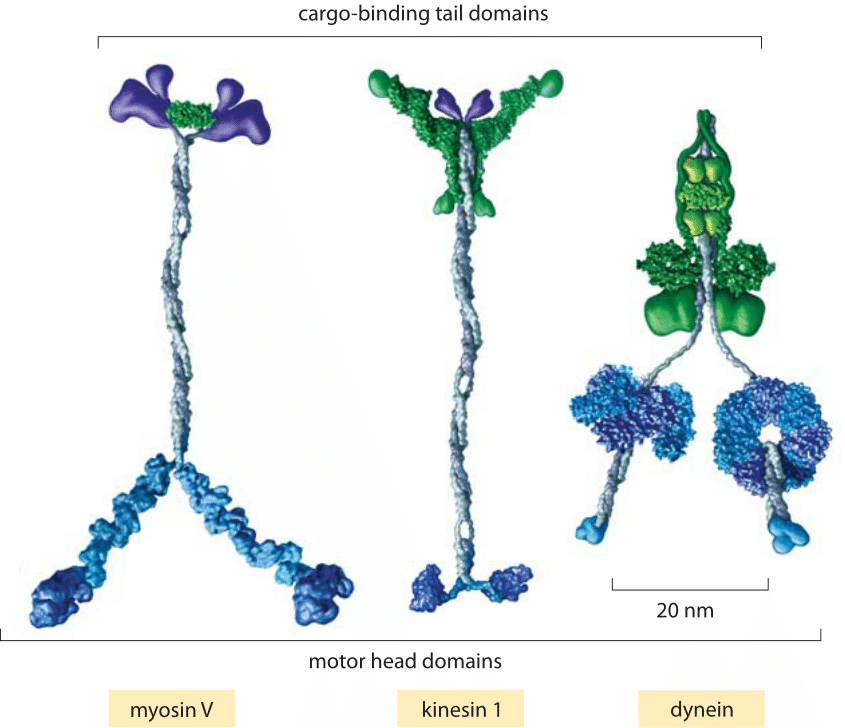
\includegraphics[width=0.5\columnwidth]{motor_comparison}
	\caption{Comparison of the three primary motor proteins (from left to right): myosin, kinesin, dynein. Image taken from \cite{philips__nodate}.}
	\label{fig:motor proteins} 
\end{figure}

Astonishingly, each of these motors is composed of two legs that combine to form a bipedal structure (see figure \ref{fig:motor proteins}). that steps like a human as it moves along the cytoskeleton. Myosin and kinesin behave like a normal person; their steps alternate between opposing domains. This motion is called \textit{hand over hand} stepping \cite{noauthor_drunk_nodate}. Dynein, however, is unique in its motion as it takes hand-over-hand steps but also \textit{inchworms} meaning that it often steps twice with the same foot. Furthermore, dynein even takes frequent backwards steps as shown in the stepping histogram in figure \ref{fig:weihong histogram} \cite{qiu_dynein_2012}. Collectively this behavior has earned dynein the title of \textit{drunken walker} which compactly summarizes its peculiar tendencies \cite{noauthor_drunk_nodate}. \\

\begin{figure}[!hbt]
	\centering
	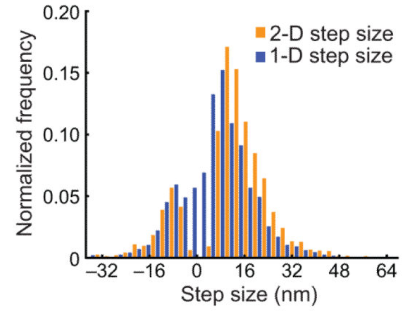
\includegraphics[width=0.5\columnwidth]{weihong_histogram}
	\caption{Stepping histogram showing the distribution of step sizes for \textit{in vitro} dynein. 1-D data corresponds to the projection of the step along the axis of the microtubule. 2-D data corresponds to the total step size over the two-dimensional structure. Figure taken form \cite{qiu_dynein_2012}.}  
	\label{fig:weihong histogram} 
\end{figure}

This unique stepping behavior makes dynein an interesting subject to study. There have been significant efforts aimed at characterizing the complex, multi-phase chemical cycle involved in the hydrolysis of ATP\cite{cianfrocco_mechanism_2015}. However, the dynamics of dynein's physical motion through space remains an open question. In this thesis, we examine a simplified physical model for the motion of dynein using Brownian dynamics. By simulating this model, we demonstrate it's ability to replicate of many observed properties of the protein. We will also use the model to comment a proposed mechanism for how dynein generates most of its movement, namely the powerstroke model. 

